%% Charlie Redmon
%% 20171020
%% SEM path diagram

% standalone class for individual image to be included in a document
% border=15pt controls the whitespace padding around the diagram
\documentclass[border=15pt]{standalone}

% additional packages
\usepackage{amsmath}

% load custom style configurations from separate file
\input{setupSEMstyle.tex}

\usetikzlibrary{positioning, calc, arrows.meta, shapes.geometric}

\tikzstyle{lv}=[shape=circle,
                draw=black!80,
                thick,
                minimum width=1.3cm]
\tikzstyle{ov}=[shape=rectangle,
                draw=black!80,
                minimum height=1.3cm,
                minimum width=1.3cm,
                thick]


\begin{document}

%% ">=Latex" sets the arrow head style
%% "semithick" sets the line width (0.6 pt)
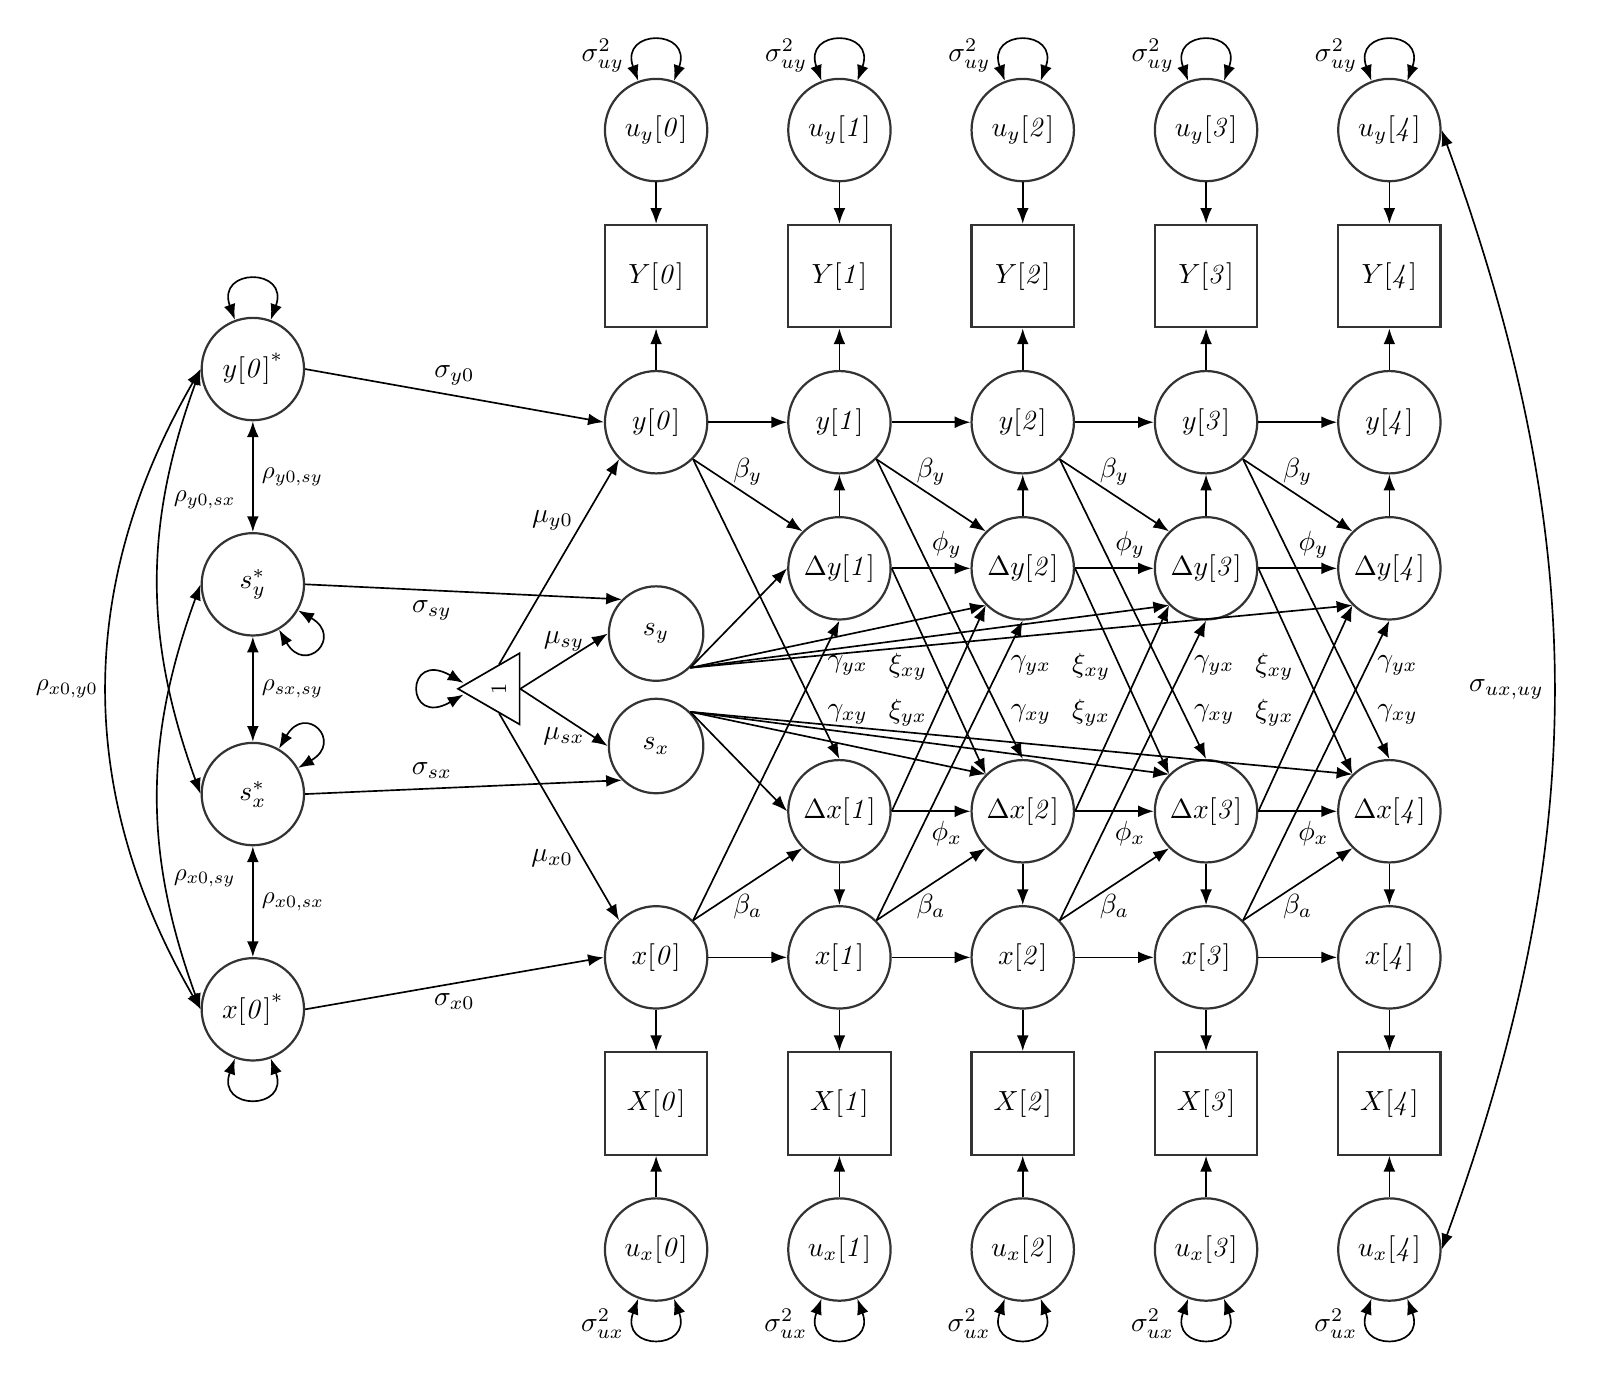
\begin{tikzpicture}[>=Latex, semithick]

% latent variables
\node[lv] (y1) at (0, 2) {$y$[\emph{1}]};
\node[lv, left=of y1] (y0) {$y$[\emph{0}]};
\node[lv, right=of y1] (y2) {$y$[\emph{2}]};
\node[lv, right=of y2] (y3) {$y$[\emph{3}]};
\node[lv, right=of y3] (y4) {$y$[\emph{4}]};
% paths
\path[->] (y0.east) edge (y1.west);
\path[->] (y1.east) edge (y2.west);
\path[->] (y2.east) edge (y3.west);
\path[->] (y3.east) edge (y4.west);

\node[lv, below=1.5em of y1] (deltY1) {$\Delta y$[\emph{1}]};
\node[lv, below=1.5em of y2] (deltY2) {$\Delta y$[\emph{2}]};
\node[lv, below=1.5em of y3] (deltY3) {$\Delta y$[\emph{3}]};
\node[lv, below=1.5em of y4] (deltY4) {$\Delta y$[\emph{4}]};

% paths
\path[->] (deltY1.east) edge node[above, pos=0.7] {$\phi_y$} (deltY2.west);
\path[->] (deltY2.east) edge node[above, pos=0.7] {$\phi_y$} (deltY3.west);
\path[->] (deltY3.east) edge node[above, pos=0.7] {$\phi_y$} (deltY4.west);

% paths
\path[->] (deltY1.north) edge (y1.south);
\path[->] (deltY2.north) edge (y2.south);
\path[->] (deltY3.north) edge (y3.south);
\path[->] (deltY4.north) edge (y4.south);

% paths
\path[->] (y0.south east) edge node[above] {$\beta_y$} (deltY1.north west);
\path[->] (y1.south east) edge node[above] {$\beta_y$} (deltY2.north west);
\path[->] (y2.south east) edge node[above] {$\beta_y$} (deltY3.north west);
\path[->] (y3.south east) edge node[above] {$\beta_y$} (deltY4.north west);

%% Xs
\node[lv, below=5em of deltY1] (deltX1) {$\Delta x$[\emph{1}]};
\node[lv, below=5em of deltY2] (deltX2) {$\Delta x$[\emph{2}]};
\node[lv, below=5em of deltY3] (deltX3) {$\Delta x$[\emph{3}]};
\node[lv, below=5em of deltY4] (deltX4) {$\Delta x$[\emph{4}]};

% paths
\path[->] (deltX1.east) edge node[below, pos=0.7] {$\phi_x$} (deltX2.west);
\path[->] (deltX2.east) edge node[below, pos=0.7] {$\phi_x$} (deltX3.west);
\path[->] (deltX3.east) edge node[below, pos=0.7] {$\phi_x$} (deltX4.west);

% x
\node[lv, below=1.5em of deltX1] (x1) {$x$[\emph{1}]};
\node[lv, left=of x1] (x0) {$x$[\emph{0}]};
\node[lv, below=1.5em of deltX2] (x2) {$x$[\emph{2}]};
\node[lv, below=1.5em of deltX3] (x3) {$x$[\emph{3}]};
\node[lv, below=1.5em of deltX4] (x4) {$x$[\emph{4}]};
% paths between x's
\path[->] (x0.east) edge (x1.west);
\path[->] (x1.east) edge (x2.west);
\path[->] (x2.east) edge (x3.west);
\path[->] (x3.east) edge (x4.west);
% paths from delta x to x
\path[->] (deltX1.south) edge (x1.north);
\path[->] (deltX2.south) edge (x2.north);
\path[->] (deltX3.south) edge (x3.north);
\path[->] (deltX4.south) edge (x4.north);
% paths from x_i to delta x_{i+1}
\path[->] (x0.north east) edge node[below] {$\beta_a$} (deltX1.south west);
\path[->] (x1.north east) edge node[below] {$\beta_a$} (deltX2.south west);
\path[->] (x2.north east) edge node[below] {$\beta_a$} (deltX3.south west);
\path[->] (x3.north east) edge node[below] {$\beta_a$} (deltX4.south west);

% paths from x_i to delta y_{i+1}
\path[->] (x0.north east) edge node[right, pos=0.85] {$\gamma_{yx}$} (deltY1.south);
\path[->] (x1.north east) edge node[right, pos=0.85] {$\gamma_{yx}$} (deltY2.south);
\path[->] (x2.north east) edge node[right, pos=0.85] {$\gamma_{yx}$} (deltY3.south);
\path[->] (x3.north east) edge node[right, pos=0.85] {$\gamma_{yx}$} (deltY4.south);

% paths from y_i to delta x_{i+1}
\path[->] (y0.south east) edge node[right, pos=0.85] {$\gamma_{xy}$} (deltX1.north);
\path[->] (y1.south east) edge node[right, pos=0.85] {$\gamma_{xy}$} (deltX2.north);
\path[->] (y2.south east) edge node[right, pos=0.85] {$\gamma_{xy}$} (deltX3.north);
\path[->] (y3.south east) edge node[right, pos=0.85] {$\gamma_{xy}$} (deltX4.north);

% paths from delta y_i to delta x_{i+1}
\path[->] (deltY1.east) edge node[left, pos=0.48] {$\xi_{xy}$}
(deltX2.north west);
\path[->] (deltY2.east) edge node[left, pos=0.48] {$\xi_{xy}$}
(deltX3.north west);
\path[->] (deltY3.east) edge node[left, pos=0.48] {$\xi_{xy}$}
(deltX4.north west);

% paths from delta x_i to delta y_{i+1}
\path[->] (deltX1.east) edge node[left, pos=0.48] {$\xi_{yx}$}
(deltY2.south west);
\path[->] (deltX2.east) edge node[left, pos=0.48] {$\xi_{yx}$}
(deltY3.south west);
\path[->] (deltX3.east) edge node[left, pos=0.48] {$\xi_{yx}$}
(deltY4.south west);

% observed variables (X)
\node[ov, below=1.5em of x0] (X0) {$X$[\emph{0}]};
\node[ov, below=1.5em of x1] (X1) {$X$[\emph{1}]};
\node[ov, below=1.5em of x2] (X2) {$X$[\emph{2}]};
\node[ov, below=1.5em of x3] (X3) {$X$[\emph{3}]};
\node[ov, below=1.5em of x4] (X4) {$X$[\emph{4}]};
% paths from x to X
\path[->] (x0.south) edge (X0.north);
\path[->] (x1.south) edge (X1.north);
\path[->] (x2.south) edge (X2.north);
\path[->] (x3.south) edge (X3.north);
\path[->] (x4.south) edge (X4.north);

% u_x variables
\node[lv, below=1.5em of X0] (ux0) {$u_x$[\emph{0}]};
\node[lv, below=1.5em of X1] (ux1) {$u_x$[\emph{1}]};
\node[lv, below=1.5em of X2] (ux2) {$u_x$[\emph{2}]};
\node[lv, below=1.5em of X3] (ux3) {$u_x$[\emph{3}]};
\node[lv, below=1.5em of X4] (ux4) {$u_x$[\emph{4}]};
% paths from u_x to X
\path[->] (ux0.north) edge (X0.south);
\path[->] (ux1.north) edge (X1.south);
\path[->] (ux2.north) edge (X2.south);
\path[->] (ux3.north) edge (X3.south);
\path[->] (ux4.north) edge (X4.south);
% ux errors
\path[<->] (ux0) edge [loop below, out=-70, in=-110,
looseness=4] node[left, xshift=-0.8em, yshift=0.5em]
{$\sigma_{ux}^2$} (ux0);
\path[<->] (ux1) edge [loop below, out=-70, in=-110,
looseness=4] node[left, xshift=-0.8em, yshift=0.5em]
{$\sigma_{ux}^2$} (ux1);
\path[<->] (ux2) edge [loop below, out=-70, in=-110,
looseness=4] node[left, xshift=-0.8em, yshift=0.5em]
{$\sigma_{ux}^2$} (ux2);
\path[<->] (ux3) edge [loop below, out=-70, in=-110,
looseness=4] node[left, xshift=-0.8em, yshift=0.5em]
{$\sigma_{ux}^2$} (ux3);
\path[<->] (ux4) edge [loop below, out=-70, in=-110,
looseness=4] node[left, xshift=-0.8em, yshift=0.5em]
{$\sigma_{ux}^2$} (ux4);


% observed variables (Y)
\node[ov, above=1.5em of y0] (Y0) {$Y$[\emph{0}]};
\node[ov, above=1.5em of y1] (Y1) {$Y$[\emph{1}]};
\node[ov, above=1.5em of y2] (Y2) {$Y$[\emph{2}]};
\node[ov, above=1.5em of y3] (Y3) {$Y$[\emph{3}]};
\node[ov, above=1.5em of y4] (Y4) {$Y$[\emph{4}]};
% paths from y to Y
\path[->] (y0.north) edge (Y0.south);
\path[->] (y1.north) edge (Y1.south);
\path[->] (y2.north) edge (Y2.south);
\path[->] (y3.north) edge (Y3.south);
\path[->] (y4.north) edge (Y4.south);

% u_y variables
\node[lv, above=1.5em of Y0] (uy0) {$u_y$[\emph{0}]};
\node[lv, above=1.5em of Y1] (uy1) {$u_y$[\emph{1}]};
\node[lv, above=1.5em of Y2] (uy2) {$u_y$[\emph{2}]};
\node[lv, above=1.5em of Y3] (uy3) {$u_y$[\emph{3}]};
\node[lv, above=1.5em of Y4] (uy4) {$u_y$[\emph{4}]};
% paths from u_y to Y
\path[->] (uy0.south) edge (Y0.north);
\path[->] (uy1.south) edge (Y1.north);
\path[->] (uy2.south) edge (Y2.north);
\path[->] (uy3.south) edge (Y3.north);
\path[->] (uy4.south) edge (Y4.north);
% u_y errors
\path[<->] (uy0) edge [loop above, out=70, in=110,
looseness=4] node[left, xshift=-0.8em, yshift=-0.5em] {$\sigma_{uy}^2$} (uy0);
\path[<->] (uy1) edge [loop above, out=70, in=110,
looseness=4] node[left, xshift=-0.8em, yshift=-0.5em]
{$\sigma_{uy}^2$} (uy1);
\path[<->] (uy2) edge [loop above, out=70, in=110,
looseness=4] node[left, xshift=-0.8em, yshift=-0.5em]
{$\sigma_{uy}^2$} (uy2);
\path[<->] (uy3) edge [loop above, out=70, in=110,
looseness=4] node[left, xshift=-0.8em, yshift=-0.5em]
{$\sigma_{uy}^2$} (uy3);
\path[<->] (uy4) edge [loop above, out=70, in=110,
looseness=4] node[left, xshift=-0.8em, yshift=-0.5em]
{$\sigma_{uy}^2$} (uy4);


% s
\node[lv, below=4em of y0, minimum width=1.2cm] (sy) {$s_y$};
\node[lv, above=4em of x0, minimum width=1.2cm] (sx) {$s_x$};
% paths from s_x to delta x
\path[->] (sx.north east) edge (deltX1.west);
\path[->] (sx.north east) edge (deltX2.north west);
\path[->] (sx.north east) edge (deltX3.north west);
\path[->] (sx.north east) edge (deltX4.north west);
% paths from s_y to delta y
\path[->] (sy.south east) edge (deltY1.west);
\path[->] (sy.south east) edge (deltY2.south west);
\path[->] (sy.south east) edge (deltY3.south west);
\path[->] (sy.south east) edge (deltY4.south west);

% intercept
\node[draw, regular polygon, regular polygon sides=3, rotate=90,
scale=0.8, below left=0.2em and 5em of sy] (int) {1};
\path[->] (int.south) edge node[above] {$\mu_{sy}$} (sy.west);
\path[->] (int.south) edge node[below] {$\mu_{sx}$} (sx.west);
\path[->] (int.east) edge node[left, pos=0.7] {$\mu_{y0}$} (y0.south west);
\path[->] (int.west) edge node[left, pos=0.7] {$\mu_{x0}$} (x0.north west);
\node[above left=0.2em and 0em of int] (err) {};
\path[<->] (err) edge [loop left, out=150, in=210, looseness=15] (err);

% s*
\node[lv, above left=3em and 7em of int] (systar) {$s_y^*$};
\node[lv, below=3.8em of systar] (sxstar) {$s_x^*$};
\path[<->] (sxstar.north) edge node[right, scale=0.9] {$\rho_{sx,sy}$} (systar.south);
\path[<->] (systar) edge [loop left, out=-30, in=-60,
looseness=5] (systar);
\path[<->] (sxstar) edge [loop left, out=30, in=60,
looseness=5] (sxstar);


% paths from s* to s
\path[->] (systar.east) edge node[below, pos=0.4] {$\sigma_{sy}$} (sy.north west);
\path[->] (sxstar.east) edge node[above, pos=0.4] {$\sigma_{sx}$} (sx.south west);

% y*
\node[lv, above=4em of systar] (ystar) {$y$[\emph{0}]\textsuperscript{*}};
\path[<->] (systar.north) edge node[right, scale=0.9] {$\rho_{y0,sy}$} (ystar.south);
\path[->] (ystar.east) edge node[above] {$\sigma_{y0}$} (y0.west);
\path[<->] (ystar) edge [loop above, out=70, in=110,
looseness=4] (ystar);

% x*
\node[lv, below=4em of sxstar] (xstar) {$x$[\emph{0}]\textsuperscript{*}};
\path[<->] (sxstar.south) edge node[right, scale=0.9] {$\rho_{x0,sx}$} (xstar.north);
\path[->] (xstar.east) edge node[below] {$\sigma_{x0}$} (x0.west);
\path[<->] (xstar) edge [loop below, out=-70, in=-110,
looseness=4] (xstar);

% cross-paths
\path[<->] (xstar.west) edge[bend left=20] node[right, pos=0.3, scale=0.9] {$\rho_{x0,sy}$} (systar.west);
\path[<->] (sxstar.west) edge[bend left=20] node[right, pos=0.7, scale=0.9] {$\rho_{y0,sx}$} (ystar.west);
\path[<->] (xstar.west) edge[bend left=30] node[left, scale=0.9] {$\rho_{x0,y0}$} (ystar.west);
\path[<->] (ux4.east) edge[bend right=20] node[left] {$\sigma_{ux,uy}$} (uy4.east);


% % paths between latent variables
% \path[<->, very thick] (f1.north east) edge [bend left=30] node[color=red,
% fill=white] {\LARGE $\boldsymbol{\Phi_{_{21}}}$} (f2.north west); 
% \path[<->] ($(f1.north east)!0.7!(f1.south east)$) edge [xshift=0.85em,
% out=-30, in=30, looseness=5] node[color=blue,fill=white] {\textbf{*1}}
% ($(f1.north east)!0.3!(f1.south east)$);
% \path[<->] ($(f2.north east)!0.7!(f2.south east)$) edge [xshift=0.85em,
% out=-30, in=30, looseness=5] node[color=blue,fill=white] {\textbf{*1}}
% ($(f2.north east)!0.3!(f2.south east)$);

% % title
% \node[color=blue] at (0.3,7.8) {\Large \textbf{Model.01}};

\end{tikzpicture}

\end{document}